%\documentclass[draft]{beamer}
\documentclass{beamer}

\mode<presentation>
{
  %\usetheme[secheader]{Boadilla}
  \usetheme{default}
}

\usepackage{calc}
%\usepackage{multimedia}
\usepackage{movie15}

\usepackage[english]{babel}

\usepackage[latin1]{inputenc}

\usepackage{times}
\usepackage[T1]{fontenc}

\newcommand{\figref}[1]{\begin{flushright}{\tiny #1 }\end{flushright}}

\title[FA Characterization]{Quantitative Analysis of Focal Adhesions in TIRF
Microscopy Images}

\author[] % (optional, use only with lots of authors)
{Matthew E. Berginski}
% - Use the \inst{?} command only if the authors have different
%   affiliation.
  
\date[Hahn Lab Meeting 8/17/2009]{Hahn Lab Meeting 8/17/2009}

\usecolortheme[RGB={2,91,173}]{structure}

\begin{document}

\begin{frame}
	\titlepage
	\begin{center}
	\includegraphics[width=0.25\textwidth]{ghost}
	\end{center}
\end{frame}

\section{Introduction}

\begin{frame}
	\frametitle{Focal What?}
	\begin{columns} 
		\column{.5\textwidth} 
		\begin{itemize}
		\item Points of contact between the substrate and cells
		\item Consist of dozens of dynamically recruited proteins
		\item Important in understanding how cells navigate and sample the environment
		\end{itemize}		

		\column{.5\textwidth}
		\includegraphics[width=\textwidth]{figures/intro/cell_cartoon}	
		\figref{Lauffenburger, DA and Horwitz, AF. Cell, 84 359--69}
		\includegraphics[width=\textwidth]{figures/intro/focal_sample}	
%		\only<1>{
%		\begin{center}
%		\begin{figure}[htbp]
%		\includegraphics[width=5cm]{figures/intro/adhesion_overview}	
%		\end{figure}
%		\end{center}
%		\figref{E. Zamir and B. Geiger, Journal of Cell Science, 2001.}
%		}
%		\only<2>{
%		\begin{center}
%		\begin{figure}[htbp]
%		\includegraphics[width=5cm]{figures/intro/Pax_closeup}
%		\end{figure}
%		\end{center}
%		\figref{E. Zamir and B. Geiger, Journal of Cell Science, 2001.}
%		}
	\end{columns} 
\end{frame}

\begin{frame}
	\frametitle{Paxillin Info/Example Movie}
	\begin{columns}
		\column{0.5\textwidth}
		\begin{itemize}
		\item Paxillin - adhesion scaffolding protein
		\item Recruited to adhesions early, remains associated
		\item Data consists of time lapse images of GFP-labeled Paxillin in 3T3 fibroblasts
		\end{itemize}
		\column{0.5\textwidth}
		\begin{center}
		\begin{figure}[htbp]
		\includegraphics[width=5cm]{figures/intro/sample_original_data_w_eric}
		\end{figure}
		\end{center}
	\end{columns}
\end{frame}

\begin{frame}
	\frametitle{Paxillin Movie Backup}
	\begin{center}
	\includegraphics[width=0.24\textwidth]{figures/finding/movie_backup/01}
	\includegraphics[width=0.24\textwidth]{figures/finding/movie_backup/02}
	\includegraphics[width=0.24\textwidth]{figures/finding/movie_backup/03}
	\includegraphics[width=0.24\textwidth]{figures/finding/movie_backup/04}
	\\
	\includegraphics[width=0.24\textwidth]{figures/finding/movie_backup/05}
	\includegraphics[width=0.24\textwidth]{figures/finding/movie_backup/06}
	\includegraphics[width=0.24\textwidth]{figures/finding/movie_backup/07}
	\includegraphics[width=0.24\textwidth]{figures/finding/movie_backup/08}
	\\
	\includegraphics[width=0.24\textwidth]{figures/finding/movie_backup/09}
	\includegraphics[width=0.24\textwidth]{figures/finding/movie_backup/10}
	\end{center}
\end{frame}

%\begin{frame}
%  \frametitle{Outline}
%  \tableofcontents
%\end{frame}

\section[Finding/Tracking]{Finding/Tracking Adhesions}

\subsection{Identifying Focal Adhesions}
\begin{frame}
	\frametitle{Methods Overview}
	\begin{columns}
	\column{0.5\textwidth}
	\begin{itemize}
%	\item Prior Methods
	\item Multistage Process
		\begin{itemize}
		\item Finding Adhesions
		\item Tracking Adhesions
		\item Collect Adhesion Properties
		\item Visualization
		\end{itemize}
	\end{itemize}
	\column{0.5\textwidth}
	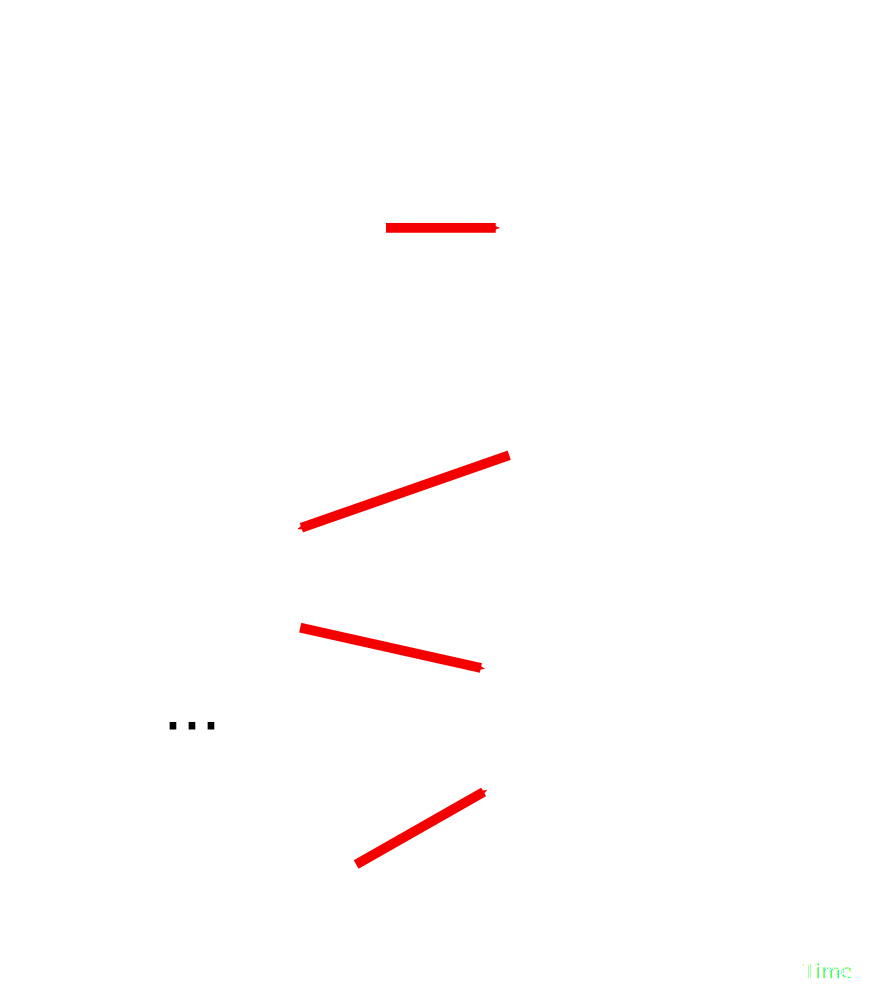
\includegraphics[width=\textwidth]{figures/finding/method_overview/overview}
	\end{columns}
\end{frame}

\begin{frame}
	\frametitle{Prior FA Analysis Methods}
	\begin{center}
	\includegraphics[width=0.8\textwidth]{figures/finding/prior}
	\end{center}
	\figref{D. Webb, et al. NCB, 6(2):154-161, 2004.}
\end{frame}

\begin{frame}
	\frametitle{Finding Adhesions}
	 \begin{itemize}
	 \item Technique adapted from E. Zamir, et al. JCS, 112(11):1655-1669, 1999.
	 \item High-pass image filter applied
	 \item Threshold used to select pixels
	 \end{itemize}
	 \bigskip
	 \begin{center}
	 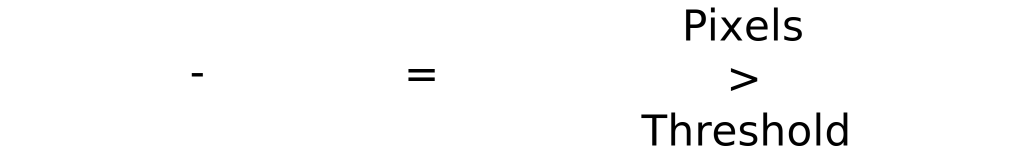
\includegraphics[width=\textwidth]{figures/finding/pixel_ID/adhesion_pixel_ID}
	 \end{center}
\end{frame}

\begin{frame}
	\frametitle{Tracking Adhesions}
	\begin{columns}
	\column{0.5\textwidth}
	\begin{itemize}
	\item Uses properties extracted from each of the images
	\item Criteria for matching adhesions between images include the percentage
	overlap and the distance between the adhesions
	\end{itemize}
	\column{0.5\textwidth}
	\includegraphics[width=\textwidth]{figures/finding/tracking_flowchart}
	\end{columns}
\end{frame}

\begin{frame}
	\frametitle{Extracted Properties Summary}
	\begin{columns}
	\column{0.33\textwidth}
	Static
		\begin{itemize}
		\item Area, Paxillin Intensity, Axial Ratio, ...
		\end{itemize}
	\column{0.33\textwidth}
	Dynamics
		\begin{itemize}
		\item Assembly and Disassembly Rates
		\end{itemize}
	\column{0.33\textwidth}
	Spatial
		\begin{itemize}
		\item Distance from Cell Edge \bigskip
		\end{itemize}
	\end{columns}
	\begin{center}
	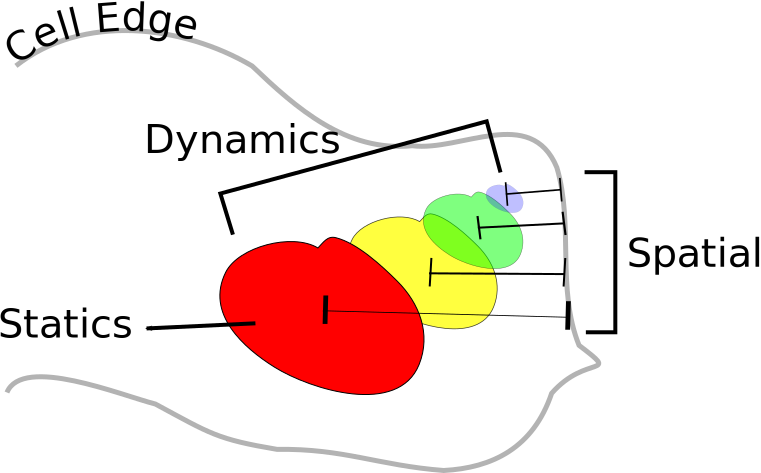
\includegraphics[width=0.8\textwidth]{figures/analysis/property_cartoon}
	\end{center}
\end{frame}

\begin{frame}
	\frametitle{Finding Assembly and Disassembly Rates}
	\begin{center}
	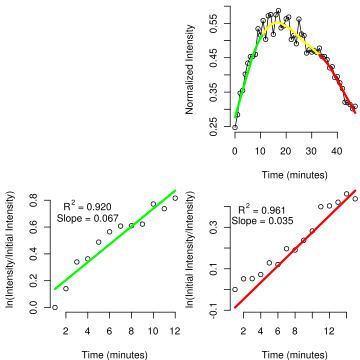
\includegraphics[height=0.85\textheight]{figures/analysis/kinetics_example.png}
	\end{center}
\end{frame}

\begin{frame}
	\frametitle{Overall Assembly and Disassembly Rates}
	\begin{center}
	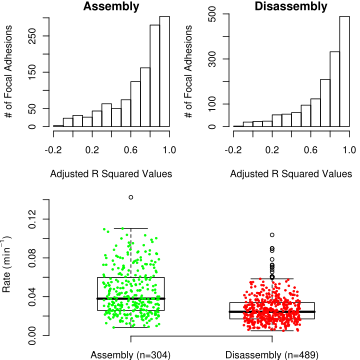
\includegraphics[height=0.85\textheight]{figures/analysis/overall_kinetics.png}
	\end{center}
\end{frame}

\begin{frame}
	\frametitle{Spatial Properties}
	\begin{center}
	\includegraphics[width=0.45\textwidth]{figures/analysis/spatial_cartoon.png}
	\\
	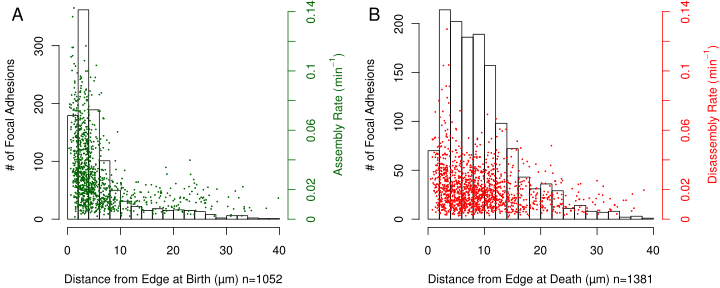
\includegraphics[width=0.9\textwidth]{figures/analysis/spatial.png}
	\end{center}
\end{frame}

\begin{frame}
	\frametitle{Visualizing the Results}
	\begin{center}
	\includegraphics[width=\textwidth]{figures/analysis/visualize_frame}
	\end{center}
\end{frame}

\begin{frame}
	\frametitle{JNK phosphorylates Paxillin on Serine 178}
	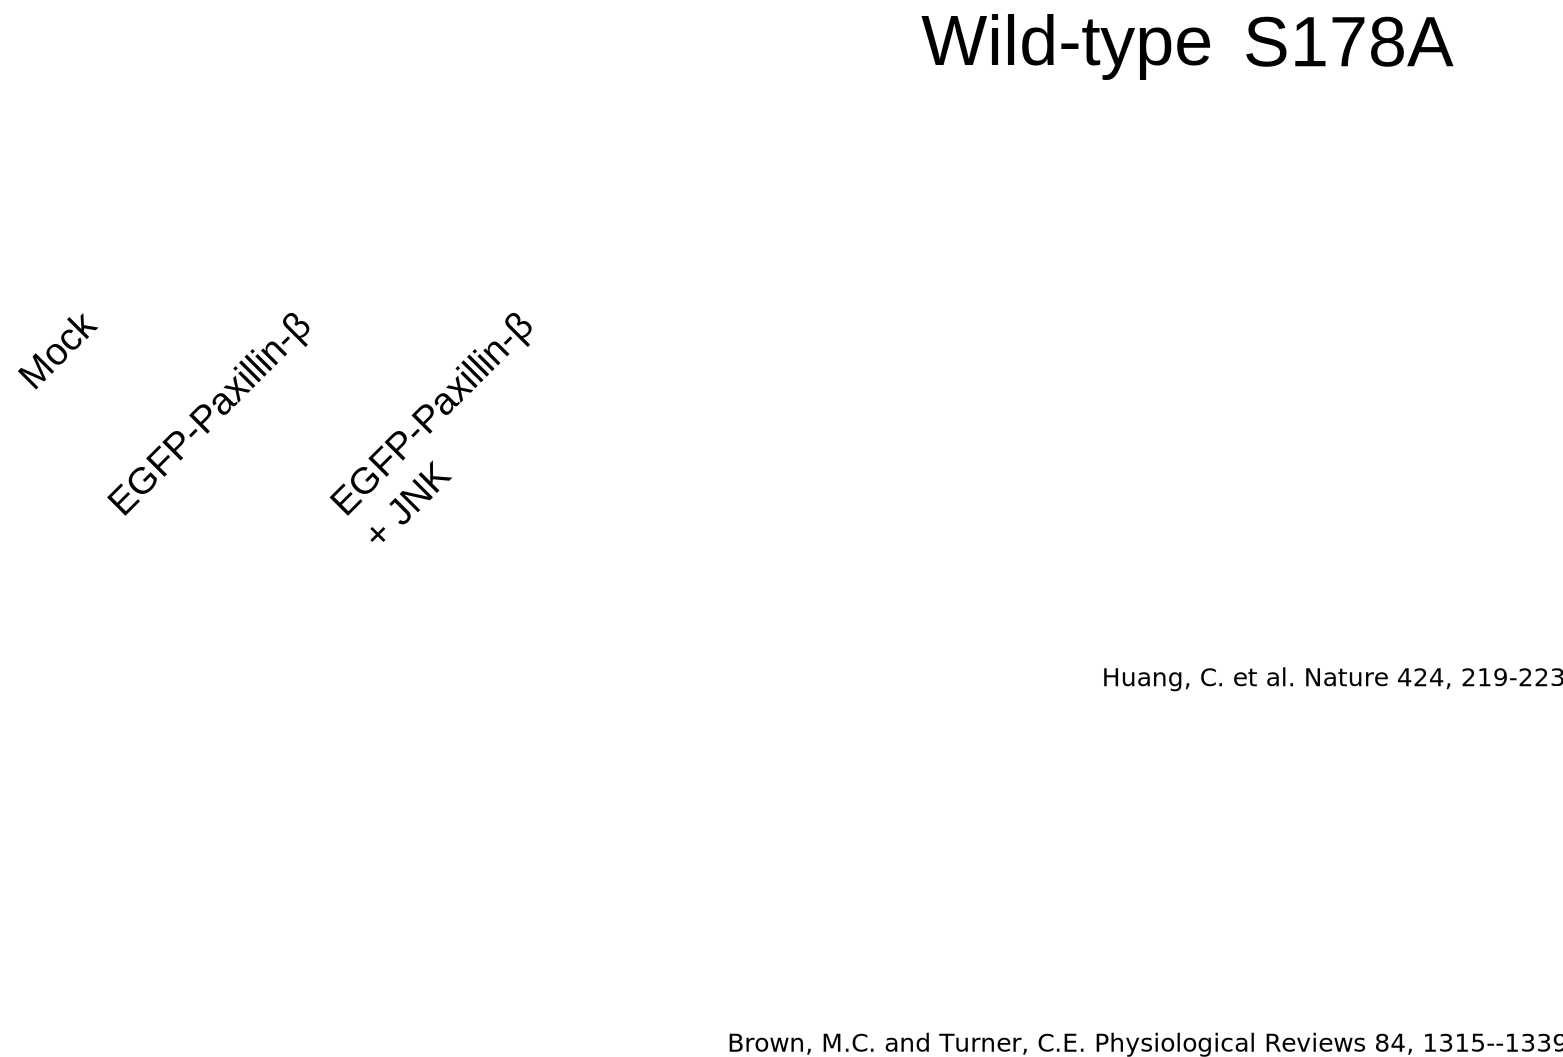
\includegraphics[height=0.8\textheight]{figures/S178A/verification/all}
\end{frame}

\begin{frame}
	\frametitle{The S178A Mutant Perturbs Adhesion Development}
	\begin{center}
	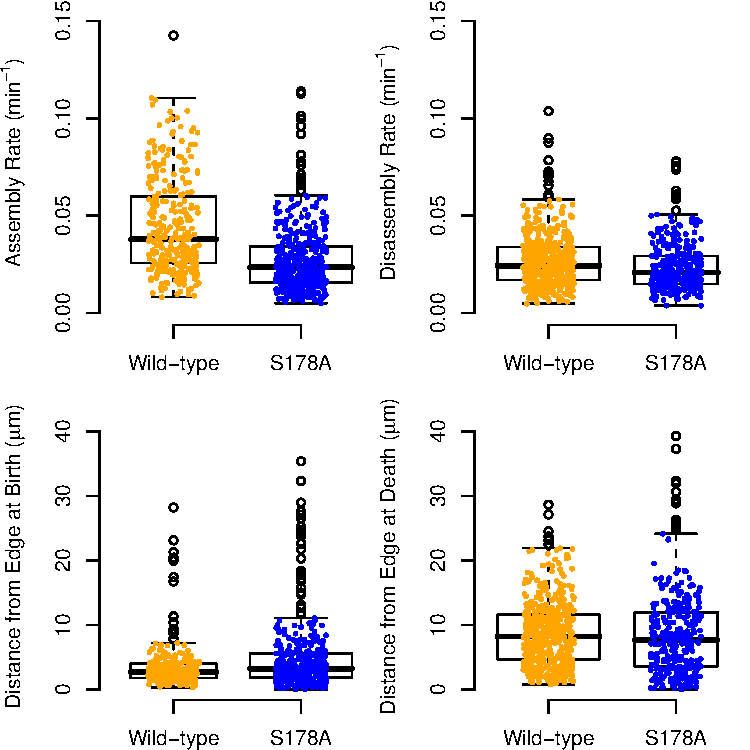
\includegraphics[height=0.8\textheight]{figures/S178A/S178A_vs_wild-type}
	\end{center}
\end{frame}

\begin{frame}
	\frametitle{The S178A Mutation Affects Phase Length Differences}
	\begin{center}
	\includegraphics[height=0.8\textheight]{figures/S178A/adhesion_phase_lifetimes}
	\end{center}
\end{frame}

\begin{frame}
	\frametitle{The S178A Mutation Affects Phase Length Differences}
	\begin{center}
	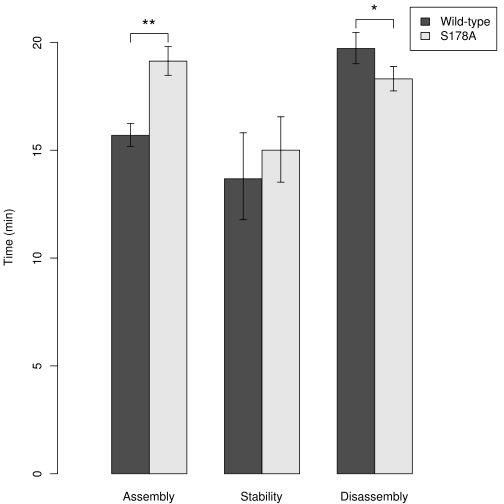
\includegraphics[height=0.8\textheight]{figures/S178A/adhesion_phase_lifetimes_alt}
	\end{center}
\end{frame}

\begin{frame}
	\frametitle{S178A Differences Summary}
	\includegraphics[width=\textwidth]{figures/S178A/sample_timecourse}
\end{frame}

\begin{frame}
	\frametitle{Future Work}
	\begin{itemize}
	\item Addition of more software features
		\begin{itemize}
		\item Integration of the cell edge velocity
		\end{itemize}
	\item Examining other signaling network perturbations
	\end{itemize}
\end{frame}

%\subsection{Tracking the Adhesions}
%
%\begin{frame}
%	\frametitle{Tracking System}
%	\begin{columns}
%		\column{0.5\textwidth}
%		\begin{itemize}
%		\item Based on a birth-death model of adhesion life
%		\item Tracking is based on adhesion centroid position and pixel overlap with adhesions in next frame
%		\end{itemize}
%		\column{0.5\textwidth}
%		\begin{center}
%		\includegraphics[height=0.75\textheight]{figures/finding/flow_charts/fa_workflow.pdf}
%		\end{center}
%	\end{columns}
%\end{frame}
%
%\subsection{Visualizing the Results}
%
%\begin{frame}
%	\frametitle{Visualizing Single Adhesions}
%	\begin{center}
%	\includegraphics[height=0.75\textheight]{figures/finding/montage_00004}
%	\end{center}
%\end{frame}
%
%\begin{frame}
%	\frametitle{Tracking Example Movie - Unique Colors}
%	\begin{center}
%	\includegraphics[width=10.88cm]{figures/finding/orig_track_sample}
%	\end{center}
%\end{frame}
%
%\begin{frame}
%	\frametitle{Tracking Example Movie - Birth Time Colors}
%	\begin{center}
%	\includegraphics[width=10.88cm]{figures/finding/time_track_sample}
%	\end{center}
%\end{frame}
%
%\section[Properties]{Adhesion Properties}
%

\end{document}
